\documentclass{usireport}

%% VARIABLES
\newcommand\namesurname{Alessandro Gobbetti}
\newcommand\assignment{Assignment 3}
\newcommand\assignmenttitle{}

\newcommand\subject{Mobile and Wearable Computing}

\begin{document}
\maketitlepage

\section{Introduction}
This is the third assignment for the Mobile and Wearable Computing course. The code is available at: \\\url{https://github.com/Alessandro-Gobbetti/Mobile-and-Wearable-Computing/tree/main/Assignment3}.

\section{New Daily Data Visualization}

The goal of this exercise is to add a new fragment to show weekly steps taken day by day. The fragment is called \texttt{DayFragment} and it is very similar to the \texttt{ReportFragment}.

A new xml layout file is created with a bar chart to show the steps taken each day of the week and a circular progress bar is shown while the data is being loaded. 
\begin{minted}{xml}
<com.anychart.AnyChartView
        android:id="@+id/dayBarChart"
        android:layout_width="match_parent"
        android:layout_height="300dp"
        app:layout_constraintBottom_toBottomOf="parent"
        app:layout_constraintEnd_toEndOf="parent"
        app:layout_constraintHorizontal_bias="0.0"
        app:layout_constraintStart_toStartOf="parent"
        app:layout_constraintTop_toTopOf="parent"
        app:layout_constraintVertical_bias="0.31" />

<com.google.android.material.progressindicator.CircularProgressIndicator
    android:id="@+id/loadingBarDay"
    android:indeterminate="true"
    android:layout_width="wrap_content"
    android:layout_height="wrap_content"
    app:layout_constraintBottom_toBottomOf="parent"
    app:layout_constraintVertical_bias="0.4"
    app:layout_constraintEnd_toEndOf="parent"
    app:layout_constraintStart_toStartOf="parent"
    app:layout_constraintTop_toTopOf="parent" />
\end{minted}

The \texttt{DayFragment} class is created to handle the fragment. It contains a method to create the chart. The method ask the database for the steps taken each day in the last week, which returns the step count for each existing day in the database. Then, it creates a map with the days of the week and loads the step count for each day. If the day is not in the database, the step count is left to 0. The map is then used to create the chart. 

\begin{minted}{java}
public class DayFragment extends Fragment {

    ...

    public Cartesian createColumnChart(){

        //***** Read data from SQLiteDatabase *********/
        // Get the map with days and number of steps for this week
        //  from the database and assign it to variable stepsByDay

        String lastWeek = new SimpleDateFormat("yyyy-MM-dd").format(
                new Date(cDate.getTime() - 7 * 24 * 3600 * 1000));
        stepsByDay = StepAppOpenHelper.loadStepsByDay(getContext(), lastWeek);

        // Creating a new map that contains days of the week from 0 to 6 and
        //  number of steps during each day set to 0
        Map<String, Integer> graph_map = new TreeMap<>();
        Date lastWeekDate = new Date(cDate.getTime() - 7 * 24 * 3600 * 1000);
        for(int i =0; i<7; i++){
            Date day = new Date(lastWeekDate.getTime() + i * 24 * 3600 * 1000);
            String dayString = new SimpleDateFormat("yyyy-MM-dd").format(day);
            graph_map.put(dayString, 0);
        }

        // Replace the number of steps for each day in graph_map
        //  with the number of steps read from the database
        graph_map.putAll(stepsByDay);

        //***** Create column chart using AnyChart library *********/
        // Create and get the cartesian coordinate system for column chart
        Cartesian cartesian = AnyChart.column();

        // Create data entries for x and y axis of the graph
        List<DataEntry> data = new ArrayList<>();

        for (Map.Entry<String,Integer> entry : graph_map.entrySet())
            data.add(new ValueDataEntry(entry.getKey(), entry.getValue()));

        // Add the data to column chart and get the columns
        Column column = cartesian.column(data);

        //***** Modify the UI of the chart *********/
        // Change the color of column chart and its border
        column.fill("#1EB980");
        column.stroke("#1EB980");


        // Modifying properties of tooltip
        column.tooltip()
                .titleFormat("At Day: {%X}")
                .format("{%Value} Steps")
                .anchor(Anchor.RIGHT_BOTTOM);

        // Modify column chart tooltip properties
        column.tooltip()
                .position(Position.RIGHT_TOP)
                .offsetX(0d)
                .offsetY(5);

        // Modifying properties of cartesian
        cartesian.tooltip().positionMode(TooltipPositionMode.POINT);
        cartesian.interactivity().hoverMode(HoverMode.BY_X);
        cartesian.yScale().minimum(0);

        // Modify the UI of the cartesian
        cartesian.yAxis(0).title("Number of steps");
        cartesian.xAxis(0).title("Day of the week");
        cartesian.background().fill("#00000000");
        cartesian.animation(true);

        return cartesian;
    }
}
\end{minted}

Finally we just have to create a function to retrieve the correct data from the database. This is done in the \texttt{StepAppOpenHelper} class. The function \texttt{loadStepsByDay} is similar to the \texttt{loadStepsByHour} function, but it retrieves the steps taken each day of the week.

\begin{minted}{java}
public static Map<String, Integer> loadStepsByDay(Context context, String date){

    // 1. Define a map to store the day and number of steps as key-value pairs
    Map<String, Integer>  map = new HashMap<>();

    // 2. Get the readable database
    StepAppOpenHelper databaseHelper = new StepAppOpenHelper(context);
    SQLiteDatabase database = databaseHelper.getReadableDatabase();

    // 3. Define the query to get the data for the last week
    Cursor cursor = database.rawQuery("SELECT day, COUNT(*)  FROM num_steps " +
            "WHERE day >= ? GROUP BY day ORDER BY  day ASC ", new String [] {date});
    // 4. Iterate over returned elements on the cursor
    cursor.moveToFirst();
    for (int index=0; index < cursor.getCount(); index++) {
        // get only the day of the week
        String tmpKey = cursor.getString(0);
        Integer tmpValue = Integer.parseInt(cursor.getString(1));

        //2. Put the data from the database into the map
        map.put(tmpKey, tmpValue);

        cursor.moveToNext();
    }

    // 5. Close the cursor and database
    cursor.close();
    database.close();

    // 6. Return the map with days and number of steps
    return map;
}
\end{minted}

\section{Results}
\autoref{fig:daily_report} shows the new fragment that displays the steps taken each day of the week. It is noticiable that a lot of steps are taken on October 30th, October 23rd has some steps, while the other days have no steps taken. 

\begin{figure}[H]
    \centering
    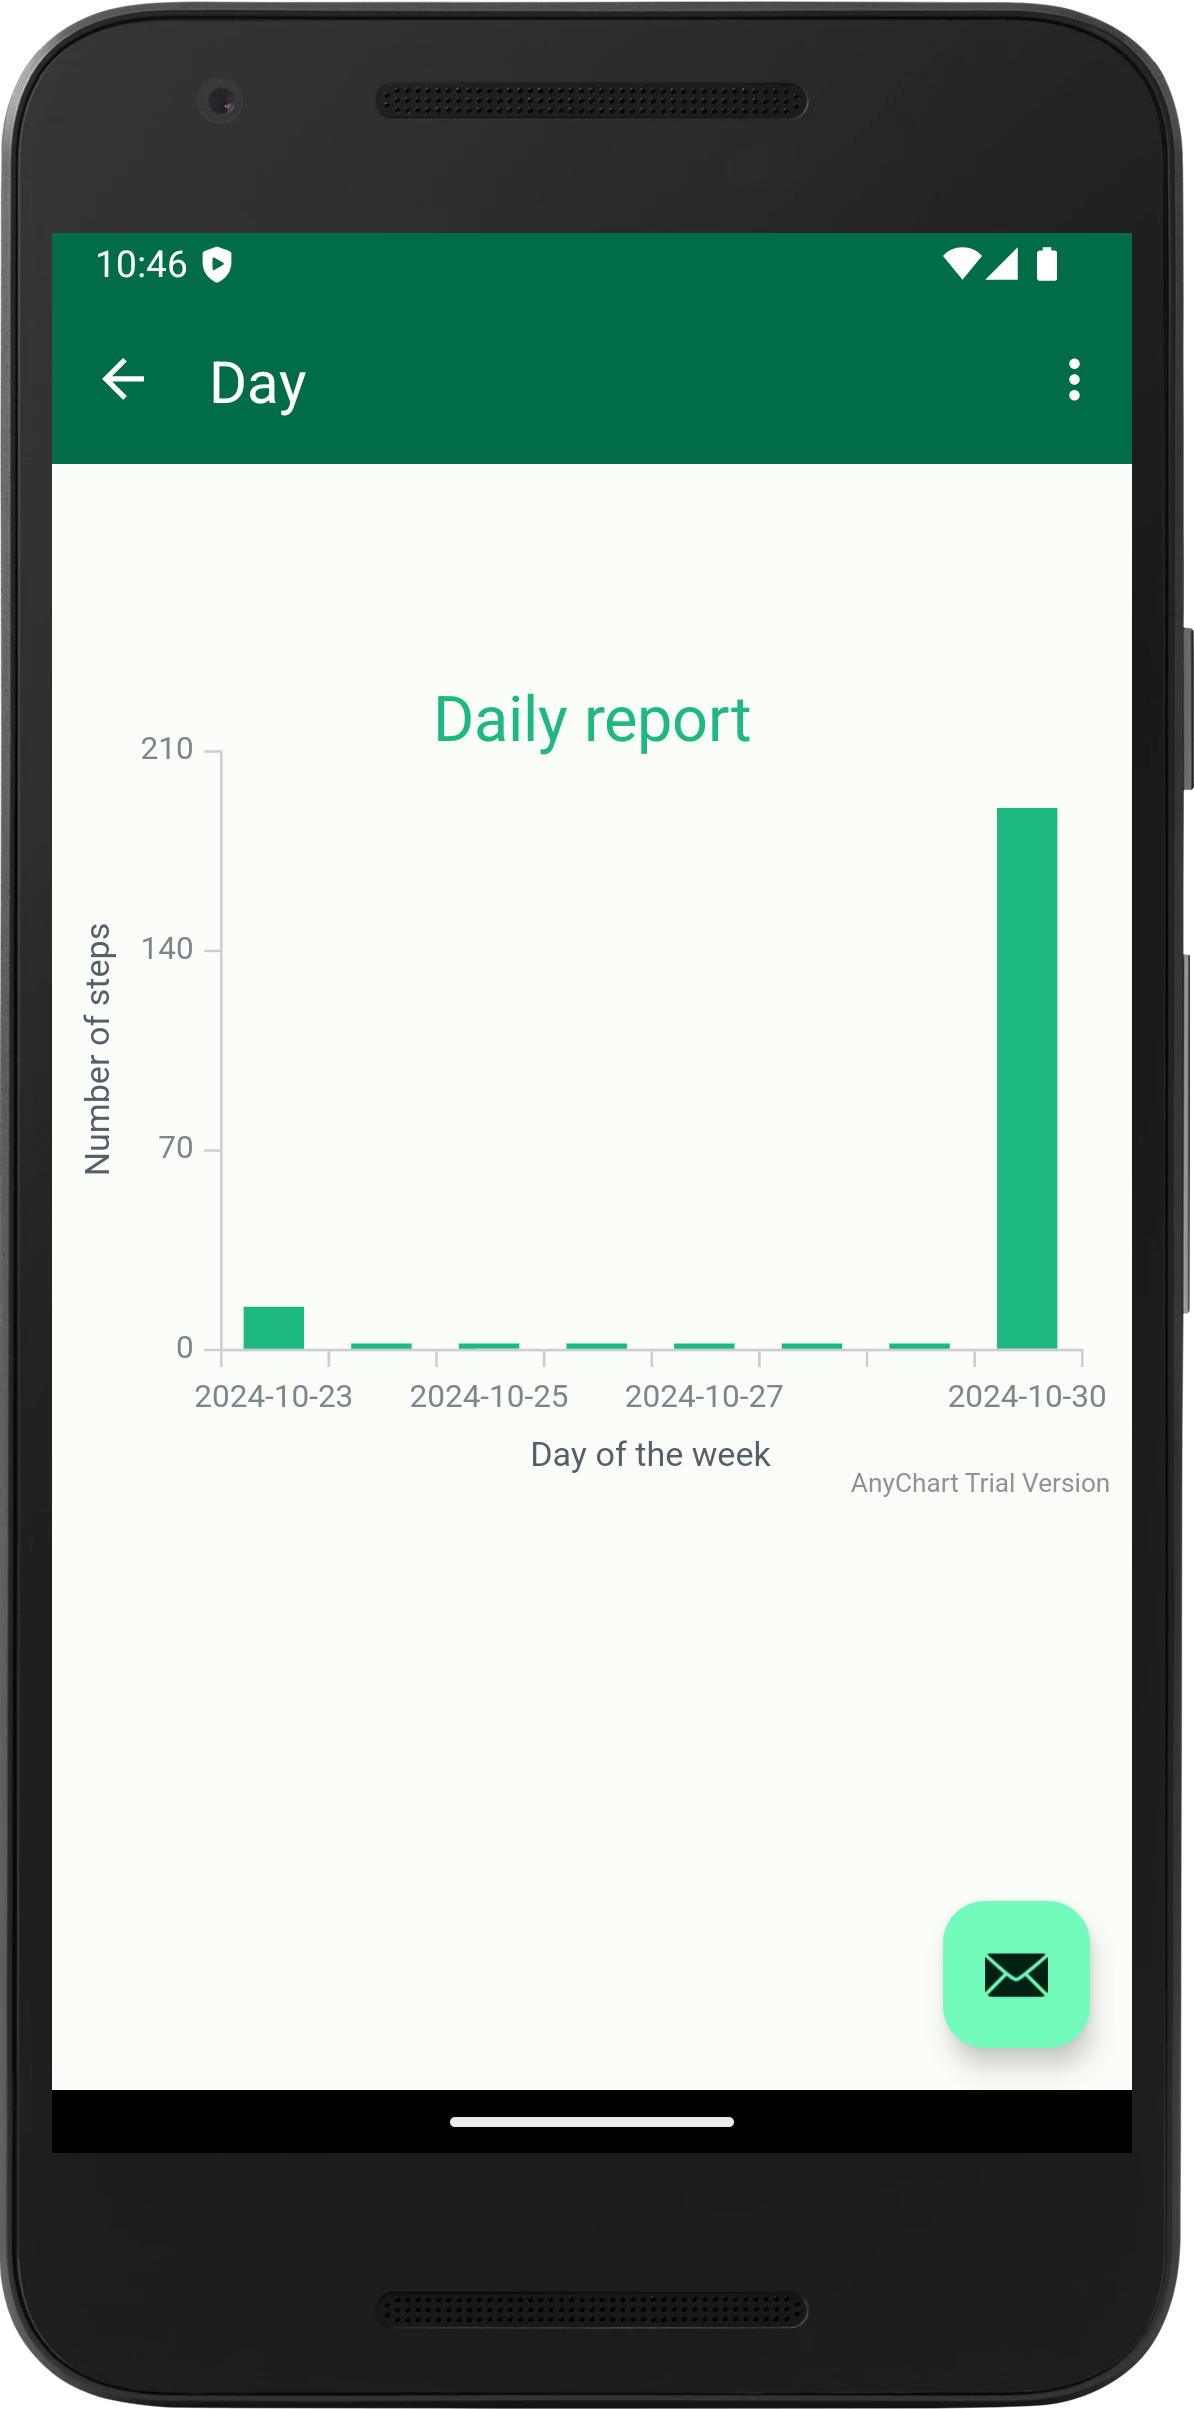
\includegraphics[width=0.3\textwidth]{fig/daily_report.png}
    \caption{Daily report}
    \label{fig:daily_report}
\end{figure}





\end{document}
